%! Author = Filippo Vissani
%! Date = 08/02/24
% !TeX root = ../thesis-main.tex

%----------------------------------------------------------------------------------------
\chapter{Evaluation}
\label{chap:evaluation}
%----------------------------------------------------------------------------------------

This chapter delves into the evaluation of the reactive extensions introduced into the Collektive framework. The chapter is divided into two main sections:

\begin{itemize}
    \item \Cref{section:testing} details the unit testing strategy employed to ensure the correctness of the implemented code. It highlights the chosen testing framework, and the testing style adopted, and showcases an example test related to the \texttt{rExchange} construct.
    \item \Cref{section:analysis-ergonomics-proposed-models} compares the usability of the DSL for implementing aggregate programs in the two proposed reactive models. To facilitate the comparison, an example program implementing the "gradient with obstacles" scenario is presented in both DSLs. This allows for a concrete side-by-side assessment of the strengths and weaknesses of each model from a usability perspective.
\end{itemize}

\section{Testing}
\label{section:testing}

To ensure the accuracy of the code developed, the project implemented a comprehensive suite of unit tests to validate the implementation. This approach not only instilled confidence in refactoring efforts but also formalized expectations regarding the language's API, enabling verification and reproducibility. Specifically, unit tests were crafted using Kotest\footnote{\url{https://kotest.io/}} framework, a widely accepted tool for automated testing in Kotlin. Among its testing styles, the project opted for \texttt{StringSpec} due to its straightforward structure, which facilitates a behavior-driven approach to test composition. The most relevant tests within the project are those that verify the behavior of the aggregate constructs.

\Cref{lst:rexchange-test} contains a test that verifies part of the behavior of the \texttt{rExchange} construct. A detailed description of the test is provided below:

\begin{itemize}
    \item line 1 defines the test name;
    \item line 2 ensures test runs sequentially within a coroutine;
    \item lines 3-5 define the aggregate result based on the execution of the aggregate program in the given aggregate context, where the ID of the device is 0 and there are no neighbors;
    \item lines 6-8 launch a concurrent job in the background where the simulation is executed;
    \item line 9 defines a delay of 100 milliseconds;
    \item line 10 cancels the job previously defined;
    \item lines 11-12 define the assertions to be executed on the result.
\end{itemize}

\lstinputlisting[float,language=kotlin,label={lst:rexchange-test},caption=Part of the test suite related to the \texttt{rExchange} construct.]{listings/rexchange-test.kt}

In the proposed tests, the behavior of the aggregate constructs is checked in various cases, the checks carried out involve:

\begin{itemize}
    \item the correct alignment of the devices;
    \item the correctness of the values exchanged by the devices;
    \item the correctness of the result of the aggregate expression.
\end{itemize}

\section{Analysis of the Ergonomics of the Proposed Models}
\label{section:analysis-ergonomics-proposed-models}

In addition to evaluating the correct functioning of the aggregate constructs with the unit tests, we want to evaluate the ergonomics of the \acp{dsl} relating to the implementations of the models in \Cref{section:prm} and \Cref{section:mrms}. The aggregate program chosen to carry out this evaluation is the gradient with obstacles, which maintains the properties of the classic gradient, but introduces obstacles into the environment. \Cref{fig:gradient-environment-and-execution} shows a graphical representation of what you want to achieve. There are three types of nodes in the environment: sources (green), obstacles (red) and defaults (blue). The objective is to calculate the distance of each node from the nearest source without considering the neighbors who are considered as obstacles. The environment used in this case is a grid with five columns and five rows, where each device is a neighbor of the nearest device in each horizontal and vertical direction. In addition, the device with ID 0 is a source node, while devices with ID 2, 7, and 12 are obstacles.

\Cref{lst:gradient-obstacles-prm} and \Cref{lst:gradient-obstacles-rmsm} present the implementation of the gradient with obstacles in the purely reactive model and in the one where only sensors and messages are reactive, respectively. In both cases the node type is defined as \texttt{StateFlow<NodeType>}, allowing to change sources and obstacles at runtime. What changes is how this flow is managed: in the purely reactive case it is used directly within the aggregate constructs, while in the other a specific simulator must be created, which reevaluates the expression as the type of node varies. As regards the use of aggregate constructs within the program, the model with reactive messages and sensors is equivalent to the proactive model, while in the purely reactive model, the use of functions for manipulating flows introduces greater complexity. Based on the results obtained, the following considerations arise:


\paragraph{Readability}

In the purely reactive model, the use of rShare, rMux, and rBranch might be less familiar to developers unfamiliar with this specific DSL. Understanding the syntax and purpose of these functions requires additional learning. The model with reactive messages and sensors utilizes familiar syntax like share and conditional statements, potentially making it easier to read and understand for developers with general programming experience.

\paragraph{Maintainability}

Composing complex logic using nested functions like rMux and rBranch can lead to nested code structures, potentially impacting maintainability as the codebase grows. In the model with reactive messages and sensors conditional statements and function calls promote a more linear and explicit flow of logic, potentially improving maintainability.

\paragraph{Flexibility}

The DSL of the purely reactive model provides dedicated functions for building reactive constructs, potentially offering more flexibility for complex reactive patterns. While offering less specialized syntax, the model with reactive messages and sensors can still achieve various reactive behaviors. However, complex reactive patterns might require more verbose code compared to the purely reactive approach.

\paragraph{Learning Curve}

The purely reactive model requires learning the specific syntax and semantics of the DSL functions, while the model with reactive messages and sensors leverages familiar programming constructs, potentially reducing the learning curve for developers with general programming experience.

\begin{figure}
    \centering
    \begin{subfigure}[b]{.15\textwidth}
        \centering
        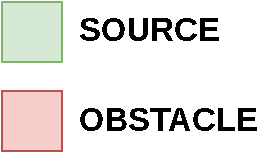
\includegraphics[width=\textwidth]{figures/gradient-environment-legend.pdf}
        \label{fig:gradient-legend}
    \end{subfigure}
    \hfill
    \begin{subfigure}[b]{.49\textwidth}
        \centering
        
\includegraphics[width=\textwidth]{figures/palette-cropped2.png}
        \label{fig:gradient-palette}
    \end{subfigure}
    \hfill
    \begin{subfigure}[b]{.49\textwidth}
        \centering
        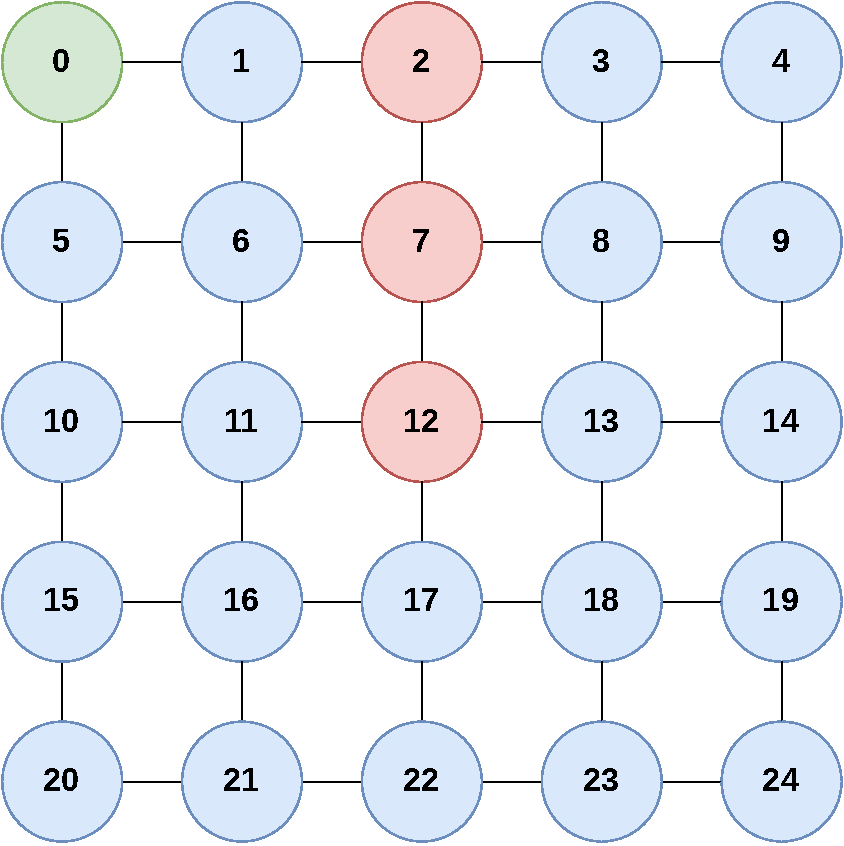
\includegraphics[width=\textwidth]{figures/gradient-environment.pdf}
        \caption{}
        \label{fig:gradient-envronment}
    \end{subfigure}
    \hfill
    \begin{subfigure}[b]{.49\textwidth}
        \centering
        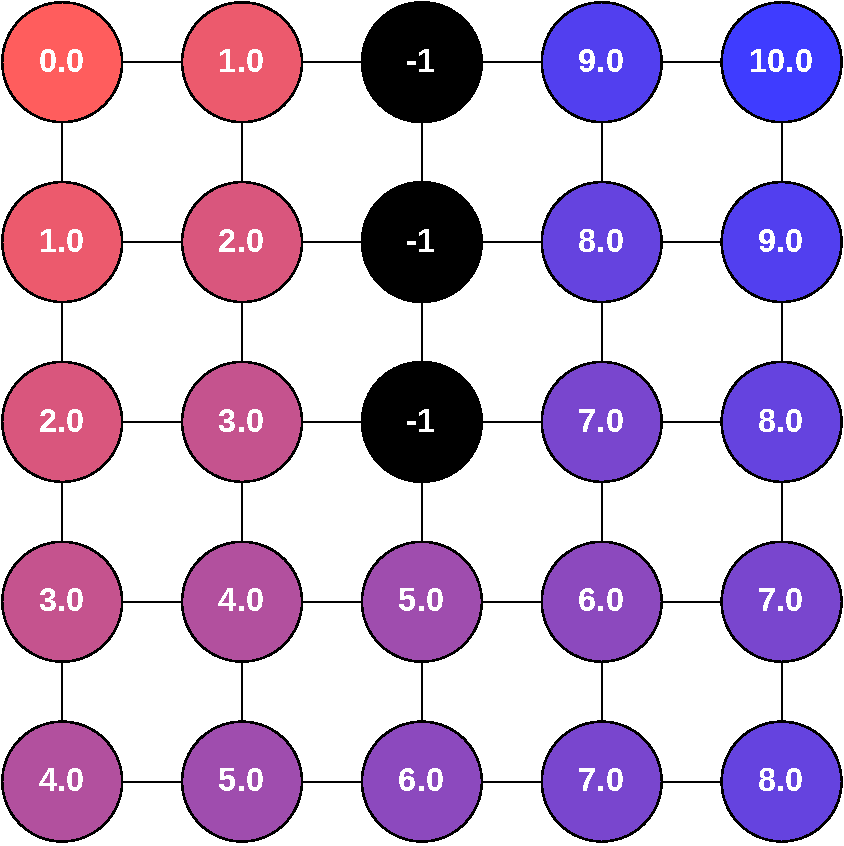
\includegraphics[width=\textwidth]{figures/gradient-environment-execution.pdf}
        \caption{}
        \label{fig:gradient-envronment-execution}
    \end{subfigure}
    \caption{\Cref{fig:gradient-envronment} presents the environment where the gradient with obstacles was executed. The node highlighted in green represents the source, while those in red represent the obstacles. \Cref{fig:gradient-envronment-execution} presents the output field of the gradient with obstacles after stabilization.}
    \label{fig:gradient-environment-and-execution}
\end{figure}

\lstinputlisting[float,language=kotlin,label={lst:gradient-obstacles-prm},caption=Gradient with obstacles implementation in purely reactive model.]{listings/gradient-obstacles-prm.kt}

\lstinputlisting[float,language=kotlin,label={lst:gradient-obstacles-rmsm},caption=Gradient with obstacles implementation in model with reactive messages and sensors.]{listings/gradient-obstacles-rmsm.kt}
